\section{Przebieg pracy}

W~tym podrozdziale opiszę fazy tworzenia projektu i~jego rozwoju.

\subsection{Przygotowanie środowiska pracy}

Pierwszym krokiem do~stworzenia systemu aukcyjnego w~technologii Ruby~on~Rails jest przygotowanie środowiska, w~którym projekt bedzie tworzony. Pominięto tutaj proces instalacji systemu operacyjnego.

\subsubsection{Instalacja narzędzi}

Większość narzędzi wymienionych w~rozdziale \ref{narzedzia} Narzędzia można zainstalować wpisując w~konsoli następujące polecenie:


\texttt{sudo apt-get install zsh screen ack-grep vim ruby git git-core tig ticgit ticgitweb sqlite3 sqlite3-dev sqliteman curl}


(Polecenie to~zadziała na~Ubuntu~11.10 oraz na~Debianie~Squeeze. Na~innych dystrybucjach zamiast \texttt{apt-get} należy użyć innego manadżera pakietów dostępnego dla danej dystrybucji. Oczywiście nazwy pakietów także mogą się różnić)

\subsubsection{Zarządzanie wersją Ruby -- RVM}

W~celu zainstalowania \textit{RVM} należy wpisać w~konsoli:


\texttt{bash -s stable < <(curl -s https://raw.github.com/wayneeseguin/rvm/master/binscripts/rvm-installer)}


Aby zainstalować Ruby w~wersji 1.9.3 należy wpisać:


\texttt{rvm install 1.9.3}


Po~konfiguracji i~kompilacji zadanej wersji Ruby należy tylko przełączyć się na~nią:


\texttt{rvm --default use 1.9.3}


Polecenie \texttt{ruby -v} powinno wypisać \texttt{ruby 1.ruby9.ruby93p0 (2011-10-30 revision 33570) [x86\_64-linux]}.

\subsubsection{Instalacja Ruby~on~Rails oraz niezbędnych wtyczek}

Ruby~on~Rails instalujemy wpisując:


\texttt{gem install rails}


W~ten sposób można już utworzyć pierwszy, podstawowy projekt Ruby~on~Rails:


\texttt{rails new auctioneer}


Polecenie to~utworzy katalog auctioneer zawierający podstawowe elementy każdego projektu Ruby~on~Rails.

\lstset{language=bash, caption=Zawartość katalogu \textit{auctioneer}, basicstyle=\ttfamily\footnotesize, captionpos=b, backgroundcolor=\color{LightGray}} \label{code.railsdir}
\begin{lstlisting}
app
app/models
app/views
app/views/layouts
app/controllers
app/helpers
app/assets
app/assets/stylesheets
app/assets/javascripts
app/assets/images
app/mailers
script
vendor
vendor/plugins
vendor/assets
vendor/assets/stylesheets
db
config
config/environments
config/locales
config/initializers
log
public
doc
test
test/integration
test/fixtures
test/functional
test/unit
test/performance
tmp
tmp/cache
tmp/cache/assets
lib
lib/tasks
lib/assets
\end{lstlisting}

Aby zainstalować konieczne do~dalszego działania wtyczki należy wyedytować plik \texttt{Gemfile} dopisując linijki z~nazwami oraz numerami wersji wtyczek.

\lstset{language=ruby, caption=Plik \texttt{Gemfile} projektu \textit{auctioneer}., basicstyle=\ttfamily\footnotesize, numbers=left, numberstyle=\footnotesize, captionpos=b, backgroundcolor=\color{LightGray}} \label{code.railsdir}
\begin{lstlisting}
source 'http://rubygems.org'

gem 'rails', '>=3.1.0'
gem 'sqlite3'

gem 'jquery-rails'
gem 'devise'
gem 'haml'
gem 'haml-rails'
gem 'formtastic'
gem 'thin'
gem 'will_paginate'
gem 'wirble', require: nil
gem 'ruby-debug19', require: nil
gem 'rspec-rails', '>= 2.6.1', group: [:development, :test]
gem 'heroku'
gem 'state_machine'

group :assets do
  gem 'sass-rails', "  ~> 3.1.0"
  gem 'coffee-rails', "~> 3.1.0"
  gem 'uglifier', '>= 1.0.3'
  gem 'therubyracer'
end

group :test do
  gem 'factory_girl_rails', '>= 1.1.0'
  gem 'cucumber-rails', '>= 1.0.2'
  gem 'capybara', '>= 1.0.1'
  gem 'database_cleaner', '>= 0.6.7'
  gem 'launchy', '>= 2.0.5'
  gem 'ruby-debug19'
  gem 'email_spec'
end
\end{lstlisting}

Po~edycji pliku \texttt{Gemfile} należy wywołać polecenie \texttt{bundle install}. Wszystkie zależności związane z~wymaganymi wtyczkami zostaną zainstalowane, a~każda zmiana w~pliku \texttt{Gemfile} wymaga ponownego uruchomienia komendy \texttt{bundle install}.

\subsubsection{Kontrola wersji Git}

W~katalogu projektu stworzonego w~poprzednim punkcie należy zainicjować system kontroli wersji wpisując polecenie:


\texttt{git init}


W~katalogu powstanie podkatalog \texttt{.git} zawierający wszystkie niezbędne informacje o historii tworzonego projektu.


W~projekcie mogą znajdować się pliki, dla~których nie chcemy przechowywać historii. Mogą to~być na~przykład pliki tymczasowe, logi, pliki backup, itp. Aby uniknąć dodawania ich do~historii rozwoju projektu należy utworzyć plik \texttt{.gitignore} i~dopisać tam niechciane pliki.


Aby zapisać bieżący stan projektu w~historii należy zaznaczyć zmiany przy pomocy polecenia \texttt{git add .} oraz wykonać commit przy pomocy \texttt{git commit}. Otworzy się domyślny edytor tekstu, w którym należy podać komentarz dotyczący zmian.

\lstset{language=bash, caption=Plik \texttt{.gitignore} projektu \textit{auctioneer}., basicstyle=\ttfamily\footnotesize, captionpos=b, backgroundcolor=\color{LightGray}} \label{code.railsdir}
\begin{lstlisting}
.sass-cache/
vendor/ruby
*~
*.swp
*.swo
tags
log/*
tmp/*
lib/mysql.rb
config/*.yml
[a-zA-Z0-9\.-_]*~
misc
capybara*
coverage
config/*.sphinx.conf
config/environments/dev_local.rb
db/sphinx/*
public/system/*
public/sitemaps/*
backup
nbproject/*
features_report.html
public/services/
public/stylesheets/all.css
public/javascripts/all.js
rerun.txt
mkmf.log
.bundle/
nohup.out
*.sqlite3
.rvmrc
doc/praca_inzynierska.pdf
\end{lstlisting}

\subsubsection{Dalsza konfiguracja}

W~poprzednich krokach została przedstawiona instalacja środowiska programistycznego dla projektu napisanego w~technologii Ruby~on~Rails. Środowisko takie jest już wystarczające i można zacząć właściwą pracę nad projektem, jednakże każde z~wyżej wymienionych narzędzi można skonfigurować według własnego uznania edytując pliki konfiguracyjne.


Do~tworzenia projektu \textit{auctioneer} użyto konfiguracji dostępnej w~repozytorium GitHub: \url{https://github.com/placek/dotfiles}.


Aby zatwierdzić taką instalację należy wykonać następujące polecenie:


\texttt{git clone git://github.com/placek/dotfiles.git; cp dotfiles/* \$HOME}

\subsection{Założenia projektu}

Zanim programista przystępuje do~pracy należy wyznaczyć szczegółowo zadania i~założenia. Wszystkie cele powinny być jasno przedstawione i~przemyślane.

\subsubsection{Założenia dotyczące projektu}

System aukcyjny powinien spełniać pewne podstawowe funkcjonalności, a~zatem powinien zapewnić możliwość:

\begin{itemize}
  \item rejestracji oraz dostępu do~konta osobom chcącym wystawiać aukcje,
  \item wystawienia aukcji oraz podania ceny minimalnej,
  \item przeglądania aukcji wraz z~ważnymi dla potencjalnych kupujących informacjami,
  \item wyszukiwania aukcji według opisu oraz podawania wyników wyszukiwania w~kolejności jaką sobie użytkownik wybierze,
  \item podbicia aukcji oraz wygrania jej na~ogólnie przyjętych zasadach.
\end{itemize}

System powinien zadbać także o~bezpieczeństwo danych użytkowników systemu oraz udostępnić możliwość administrowania danymi przez osoby uprawnione (administratorzy).

\subsubsection{Przypadki użycia i scenariusze}

Wyróżniono następujących aktorów:

\begin{enumerate}
  \item \textit{Gość} -- odwiedzający serwis \textit{auctioneer}, nie mający na~nim osobistego konta (nie zalogowany, nie zarejestrowany). Gość może przeglądać wystawione aukcje oraz wyszukiwać z~pośród nich  interesujące go~pozycje. Gość może także zarejestrować się.
  \item \textit{Użytkownik} -- aktor posiadający osobiste konto w~serwisie \textit{auctioneer}, logujący się za~pomocą adresu email oraz hasła. Użytkownik może wykonywać akcje gościa (przeglądanie wystawionych aukcji, ich wyszukiwanie). Ponadto użytkownik posiada możliwość licytowania aukcji, wystawiana własnych aukcji i~zarządzania nimi (edycja, usuwanie, zmiana stanu aukcji).
  \item \textit{Administrator} -- aktor posiadający najwyższe uprawnienia. Może zarządzać kontami innych administratorów, jak i~kontami użytkowników (dodawanie, usuwanie kont, logowanie na~konta). Administrator ma~także pełen dostęp do~wszystkich aukcji -- może je~edytować, usuwać, zmieniać ich stan.
\end{enumerate}

Wyróżniono także następujące przypadki użycia (patrz rysunek \ref{usecase}):

\begin{enumerate}
  \item \textit{Przeglądanie wystawionych aukcji} -- podstawowa funkcjonalność systemu aukcyjnego. Każdy aktor odwiedzający serwis \textit{auctioneer} powinien mieć możliwość dostępu do~listy wystawionych aukcji oraz ich szczegółowych opisów.
  \item \textit{Wyszukiwanie aukcji pod warunkiem kryteriów wyszukiwania} -- duża ilość wystawionych aukcji może spowodować problemy ze znalezieniem interesującego odwiedzającego stronę przedmiotu aukcji. Aukcje powinny być wyszukiwane ze~względu na~nazwę i opis aukcji. Powinna być także możliwość sortowania wyników według nazwy i~ceny.
  \item \textit{Rejestracja} -- odwiedzający serwis \textit{auctioneer}, nie posiadający na~nim konta osobistego powinien mieć możliwość rejestracji. Rejestracja powinna odbywać się przy użyciu adresu email nowego użytkownika oraz hasła. Aby nowo zarejestrowane konto było aktywne (można się na~nie zalogować) należy aktywować je~poprzez wykonanie instrukcji przysłanych na~email podany podczas rejestracji.
  \item \textit{Wystawianie aukcji} -- nowo utworzona aukcja powinna zawierać tytuł (będący krótkim opisem aukcji), szczegółowy opis aukcji (detale) oraz cenę minimalną. Tak przygotowana aukcja może zostać wystawiona (upubliczniona).
  \item \textit{Licytacja} -- wystawiona aukcja zgodnie z~zamiarem wystawiającego ją~powinna posiadać cenę minimalną, od~której zaczyna się licytacja. Licytacja powinna mieć termin ważności (w~założeniu -- siedem dni od~wystawienia aukcji), po którym to wyłoniony zostaje zwycięzca aukcji -- osoba, która wylicytowała najwyższą sumę. Alternatywnym zakończeniem aukcji może być przerwanie jej przez wystawiającego przed terminem ważności.
  \item \textit{Zarządzanie aukcjami użytkownika} -- użytkownik powinien mieć możliwość edycji bądź usunięcia własnych aukcji. Powinien także mieć możliwość zmiany jej stanu (wystawienie, zamknięcie aukcji, ponowne jej wystawienie).
  \item \textit{Zarządzanie administratorami} -- aktualny administrator powinien mieć możliwość dodawania oraz usuwania innych administratorów.
  \item \textit{Zarządzanie użytkownikami} -- administrator powinien mieć możliwość edycji i~usuwania użytkowników, powinien też mieć możliwość zalogowania się jako użytkownik.
  \item \textit{Zarządzanie aukcjami} -- administrator powinien posiadać dostęp do wszystkich aukcji i~mieć możliwość ich edycji, usunięcia oraz zmiany stanu.
\end{enumerate}

\begin{figure}[hbt]
  \begin{center}
    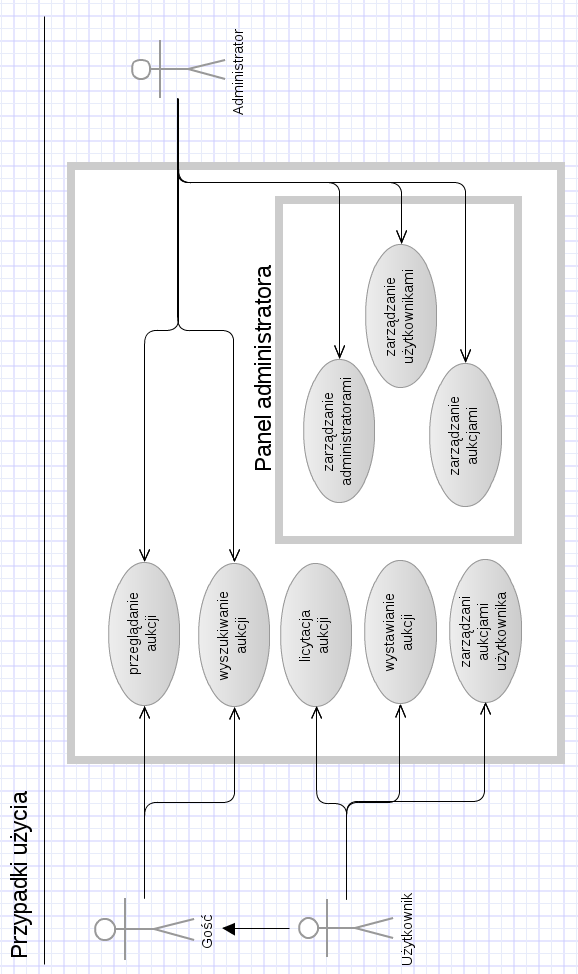
\includegraphics[height=0.8\textheight]{obrazki/usecase.png}
  \end{center}
  \caption{Diagram UML obrazujący przypadki użycia oraz aktorów.}
  \label{usecase}
\end{figure}

Wszystkie wyżej wymienione przypadki użycia powinny być zaimplementowane i~przetestowane. W~tym celu tworzone są testy behawioralne przy użyciu narzędzia \texttt{cucumber}. Testy te~przyjmują formę scenariuszy dla konkretnych przypadków użycia.

\lstset{language=sh, caption=Przykładowy scenariusz opisujący proces rejestracji nowego użytkownika., basicstyle=\ttfamily\footnotesize, numbers=left, numberstyle=\footnotesize, captionpos=b, backgroundcolor=\color{LightGray}} \label{code.simpleruby}
\begin{lstlisting}
Scenario: Registering a user account
  Given I am on the home page
  And no emails have been sent
  When I follow "Sign up"
  And I fill in the following:
    | user_email                 | user@example.com |
    | user_password              | monkey           |
    | user_password_confirmation | monkey           |
  And I press "Sign up"
  Then "user@example.com" should receive an email
  When "user@example.com" opens the email
  Then I should see "Confirmation instructions" in the email subject
  And I should see "You can confirm your account through the link below" in the email body
  And I should see "Confirm my account" in the email body
  When I follow "Confirm my account" in the email
  And I should see "Sign out"
\end{lstlisting}

\newpage

\subsection{Zadania i~ich realizacja}

Zadania, które należało wykonać aby zaimplementować system \textit{auctioner}:

\begin{enumerate}
  \item inicjacja środowiska -- zainstalowanie niezbędnych narzędzi, konfiguracja środowiska oraz stworzenie nowego projektu Ruby~on~Rails;
  \item konfiguracja projektu Ruby~on~Rails -- podpięcie wtyczek (gem), ustawienia konfiguracyjne dla projektu, utworzenie repozytorium \textit{Git} projektu, wykonanie czynności mających na~celu przygotowanie projektu dla realizacji jego architektury i~funkcjonalności;
  \item przygotowanie aplikacji na~możliwość obsługi wielu wersji językowych;
  \item utworzenie modeli użytkowników i~administratorów -- utworzenie schematu tabeli w~bazie danych, implementacja klas opakowujących, utworzenie prostych kontrolerów zarządzających modelami;
  \item dodanie funkcjonalności rejestracji/logowania -- podpięcie systemu autentykacji do istniejących modeli użytkownika i~administratora, utworzenie widoków dla funkcjonalności rejestracji, logowania, przypomnienia hasła, aktywacji konta oraz przygotowanie wersji językowych dla funkcjonalności;
  \item utworzenie modelu dla aukcji -- przygotowanie schematu dla bazy danych, utworzenie zależności pomiędzy modelami aukcji i użytkownika, utworzenie kontrolerów zarządzających aukcjami, utworzenie widoków dla aukcji, utworzenie ścieżek wywołań;
  \item dodanie możliwości wyszukiwania -- implementacja systemu zapytań do~bazy danych, obsługa tworzonych kwerend;
  \item utworzenie systemu publikacji i~podbijania aukcji -- dodanie maszyny stanów dla modelu aukcji, implementacja kontrolerów zarządzających zmianami stanu, zmiany w widokach dla funkcjonalności;
\end{enumerate}

\lstset{language=sh, caption=Lista zadań w~aplikacji \textit{ticgit}., basicstyle=\ttfamily\footnotesize, numbers=left, numberstyle=\footnotesize, captionpos=b, backgroundcolor=\color{LightGray}} \label{code.simpleruby}
\begin{lstlisting}
TicId  Title                        State   Date  Assgn    Tags
------------------------------------------------------------------------
69418c Create a new rails projec... reso... 11/07 placek   environment
36ce13 Prepare L10n and I18n env... reso... 11/07 placek   environment
fca367 Prepare a devise models f... reso... 11/07 placek   users
ed753d Create model for auction;... reso... 11/07 placek
b2296e Prepare a publication sys... reso... 11/07 placek   auction,state
\end{lstlisting}
